\documentclass[solid,math,chem,code,plot,gloss]{bmc}

\titlehead{Bespoke Multipurpose Class}
\title{\texorpdfstring{BMC \hfill \fontsize{1.35cm}{1.35cm}\fontseries{t}\selectfont \emph{v}0.2.2*}{BMC v0.2.2*}}
\subtitle{Pretentiousness Given Form}
\author{tecosaur \footnotesize \newline of GitHub}

\usepackage[symbol*]{footmisc}
\renewcommand{\thefootnote}{\fnsymbol{footnote}}
\usepackage[normalem]{ulem}

\newcommand*{\fullref}[1]{\hyperref[{#1}]{\ref*{#1} \nameref*{#1}}}

\usepackage[style=apa,backend=biber]{biblatex}
\bibliography{refs}

\begin{document}

\newglossaryentry{tracking}
{
    name=tracking,
    description={Tracking is the typographer's term for letter-spacing. Tracking adjusts the letter-spacing uniformly over a range of characters.}
}

\maketitle

\thispdfpagelabel{Preface}
\section*{Preface}

\vspace{1cm}

Like with most things I didn't start out with the intent to end up this way.
Initially I had a slowly growing template that I used for most documents;
every so often I'd discover a package that did something I liked,
or a setting that I preferred to be non-default.
\emph{Every} time that happened I'd want to go through the current documents
I was working on and apply the latest revelations.
Then when revisiting old documents I'd want to get them `up to scratch'.
There would always be the odd document I forgot about, or line missed,
and so I quickly became tired of this process.

After realising that if I made a class and shoved it in my \verb|texmf|
directory that I'd be able to as many improvements as I like and they'd all
be applied when I recompiled, \emph{as well} as make initial configuration
greatly simplified --- I couldn't see a reason not to do it.

This class is very much written with my personal taste, and specific use case in mind.
While I try to keep things general it is very much built around my particular perspective.
As such it is reasonable to think that to the community as a whole the
self-importance in the name is a tad exaggerated or undeserved.
Considering that is also designed to not just convey information but also
designed to visually impress, the tagline `Pretentiousness given form''
seems somewhat appropriate.

I'm pleased to say that I consider this a project a success (in those respects).
As I have largely drawn upon snippets of LaTeX floating around online
I though the least I could do is give others that same opportunity.
As such here you have an overview of my personal class
designed to work for all of the documents I produce.
In other words a \emph{bespoke, multipurpose class} --- or \acr{BMC} for short.

\vspace{1cm}

Enjoy!

\vfill

tecosaur

\vspace{3cm}

\newpage
\fancytoc{}

\chapter{What This Does}

\section{Typography}

\subsection{Typefaces}

This package loads three typefaces.
\begin{enumerate}
    \item IBM Plex Serf
    \item IBM Plex Sans
    \item IBM Plex Mono
\end{enumerate}
I wanted a selection where serif, sans, and mono all mix well.
Ideally with a few weight variants.
Additionally I wanted a typographic style that meshed well with the
large class of documents I indented to use this for. IBM Plex seems like a good fit
(For more info see \fullref{sec:why-typefaces}). For all three of these a linespread
of 1.15 is used.

\newcommand\setrow[1]{\gdef\rowmac{#1}#1\ignorespaces}
\newcommand\clearrow{\global\let\rowmac\relax}
\clearrow
\begin{table}[!htb]
    \centering
    \setlength{\tabcolsep}{4pt}
    \begin{tabular}{
        l
        >{\rowmac\ifbool{tabularTitleRow}{}{\fontseries{b}\selectfont}}l
        >{\rowmac\ifbool{tabularTitleRow}{}{\fontseries{sb}\selectfont}}l
        >{\rowmac\ifbool{tabularTitleRow}{}{\fontseries{mb}\selectfont}}l
        >{\rowmac\ifbool{tabularTitleRow}{}{\fontseries{tx}\selectfont}}l
        >{\rowmac}l
        >{\rowmac\ifbool{tabularTitleRow}{}{\fontseries{l}\selectfont}}l
        >{\rowmac\ifbool{tabularTitleRow}{}{\fontseries{el}\selectfont}}l
        >{\rowmac\ifbool{tabularTitleRow}{}{\fontseries{t}\selectfont}}l
        }
        \toprule
        Typeface & Bold & Semibold & Medium & Text & Regular & Light & Extra L & Thin \\
        \setrow{\ttfamily\scriptsize}\verb|\selectfont| & b & sb & mb & tx & m & l & el & t \\
        \midrule
        \setrow{\rmfamily}\!Plex Serif & Words & Words & Words & Words & Words & Words & Words & Words \\
        \setrow{\rmfamily\itshape}\!Plex Serif & Words & Words & Words & Words & Words & Words & Words & Words \\
        \arrayrulecolor{page}\midrule
        \setrow{\sffamily}Plex Sans & Words & Words & Words & Words & Words & Words & Words & Words \\
        \setrow{\sffamily\itshape}Plex Sans & Words & Words & Words & Words & Words & Words & Words & Words \\
        \midrule
        \setrow{\plexsanscondensed}Condensed & Words & Words & Words & Words & Words & Words & Words & Words \\
        \setrow{\plexsanscondensed\itshape}Condensed & Words & Words & Words & Words & Words & Words & Words & Words \\
        \midrule\arrayrulecolor{text}
        \setrow{\ttfamily}Plex Mono & Words & Words & Words & Words & Words & Words & Words & Words \\
        \setrow{\ttfamily\itshape}Plex Mono & Words & Words & Words & Words & Words & Words & Words & Words \\
        \bottomrule
    \end{tabular}
    \caption{IBM Plex; Font Styles and Weights}
    \label{table:font-styles}
\end{table}

\begin{info}[][Some Typeface Considerations][tf-consid]
    While this is the default, you can still load another font as
    usual in the preamble, e.g.
    \mintinline{tex}{\usepackage{lmodern}}
    to switch to Latin Modern.
    Bear in mind that varying font weights are using throughout
    this class, so a font without the \mintinline{tex}{sb},
    \mintinline{tex}{tx}, etc.\ weights will report warnings
    along the lines of \mintinline{text}{Font shape `T1/FONT_HERE/STYLE/n' undefined}.
\end{info}

\subsection{Roman Numerals}

While biblatex does provide handy roman numeral command,
it's nice to have them available regardless.
Hence this class provides them if they aren't already available.
To get upper case roman numerals use \mintinline{tex}{\RN{1978}}
to produce \RN{1978}, and \mintinline{tex}{\Rn{1978}}
to produce \Rn{1978}.

\begin{minted}[firstnumber=304]{tex}
        \providecommand*{\RN}[1]{\expandafter\@slowromancap\romannumeral #1@}
        \providecommand*{\Rn}[1]{\romannumeral#1\relax}
\end{minted}

\subsection{Faux Small Caps}
Some fonts (such as IBM Plex) are not kind enough to provide small caps.
Simply using downscaled capitals is a barbaric and decidedly inferior solution.
So \mintinline{tex}{\fauxsc{}} is defined which, while not as nice as \emph{true}
small caps, is a darn sight better than just reducing the font size.
\mintinline{tex}{\fauxsc{}} is \emph{automatically} used when \mintinline{tex}{\textsc{}}
is called if the current font does not have small caps.
\vspace{-6pt}
\begin{center}
    \parbox{0cm}{
        \begin{tabbing}
            \texttt{\small \textbackslash textsc} using \texttt{\small \textbackslash fauxsc}:\quad \= \textsc{Small Caps} \\
            Barbaric Solution: \> S{\footnotesize MALL} C{\footnotesize APS}
        \end{tabbing}}
\end{center}

\begin{warning}[Small Caps][Usage Warning][sc-usage]
    If using this in macros or the like,
    you may get errors such as
    {\ttfamily\small ``Improper alphabetic constant''},
    {\ttfamily\small ``Missing = inserted for \texttt{\small \textbackslash ifnum}''},
    and {\ttfamily\small ``Missing number, treated \\ as zero''}.

    Here you will likely need to use
    \texttt{\small \textbackslash expandafter\textbackslash textsc\textbackslash expandafter} instead.
\end{warning}

\subsection{Penalties}
The class sets new penalties.
\begin{minted}[firstnumber=209]{tex}
    \@beginparpenalty=10000 % don't like it when a paragraph title is on a different page to the start of the content
    \hyphenpenalty=500 % not a huge fan of hyphens, but they are worthwhile
    \lefthyphenmin=2
    \righthyphenmin=3
\end{minted}

\subsection{Captions}
Caption labels are made to be upright sans-serif in the `text' style,
while captions are italic in the style of the body.
When captions flow beyond a single line, ragged right alignment is used.

\begin{minted}[firstnumber=464]{tex}
    \setkomafont{caption}{\itshape\color{text}}
    \setkomafont{captionlabel}{\fontfamily{\headingsFont}\fontseries{tx}\selectfont\upshape\color{text}}
    \captionsetup{justification=raggedright,singlelinecheck=true}
\end{minted}

\subsection{Terms and Acronyms}
With the \mintinline{tex}{gloss} option, this class loads and configures the
\mintinline{tex}{glossaries} package. Three things are changed
\newacronym{bmc}{BMC}{Bespoke Multipurpose Class}
\begin{enumerate}
    \item A new command \mintinline{tex}{\acr{TEXT}} is added. This
    \begin{enumerate}
        \item Selects the next higher font weight
        \item Scales the text vertically by a factor of 0.84, and horizontally by 0.91
        \item Increases \gls{tracking} by 7\acr{M}/100\footnote{See \P~2.1.6 of~\cite{Bringhurst_2004}}
    \end{enumerate}
    \item Acronyms are typeset in the style of \mintinline{tex}{\acr}, e.g. \gls{bmc}
    \item The glossary style in configured to a variant of \mintinline{tex}{long3col}
    \item A new command \mintinline{tex}{\newdefinedacronym{label}{short}{long}{description}} is added
\end{enumerate}

\section{Boxes}

A collection of boxed environments are defined using \mintinline{tex}{tcolorbox},
there have been two so far: \autoref{info:tf-consid} and \autoref{warn:sc-usage}.
You can use these environments like so:
\begin{minted}{tex}
    \begin{example}
        This is an example. The next one is \autoref{eg:box-demo}.
    \end{example}
\end{minted}
\begin{example}
    This is an example. The next one is \autoref{eg:box-demo}.
\end{example}
These environments also accept three optional arguments.
\begin{enumerate}
    \item The subtitle. This appears after the bold title ({\sffamily\fontseries{sb}\selectfont Example N}).
    \item The title, if this is set the counter value is shown in the right corner,
    as seen in the example below.
    \item The label suffix, defaulting to the counter value.
    The full label is \mintinline{tex}{<prefix>:<suffix>}.
\end{enumerate}
\begin{minted}{tex}
    \begin{example}[sub-title][title][box-demo]
        This is another example, following up from \autoref{eg:1}.
    \end{example}
\end{minted}
\begin{example}[sub-title][title][box-demo]
    This is another example, following up from \autoref{eg:1}.
\end{example}

A decent variety of environments are already defined (see \autoref{table:boxed-envs} and \autoref{table:boxed-envs-maths}).

\begin{table}[!htb]
    \centering
    \begin{tabular}{clll}
        \toprule
        Icon & Environment Name & Title & Label Prefix \\
        \midrule
        \renewcommand{\arraystretch}{1.5}
        \faAbstractIcon{exampleColor}{\faClipboard} \faAbstractIcon{page}{\faClipboard}[exampleColor!70!page]
        & \ttfamily\small  example & Example & \ttfamily\small eg:\\
        \faAbstractIcon{criticalColor}{\faTimes} \faAbstractIcon{page}{\faTimes}[criticalColor!70!page]
        & \ttfamily\small  critical & Critical & \ttfamily\small crit:\\
        \faAbstractIcon{questionColor}{\faQuestion} \faAbstractIcon{page}{\faQuestion}[questionColor!70!page]
        & \ttfamily\small  question & Question & \ttfamily\small qu:\\
        \faAbstractIcon{informationColor}{\faInfo} \faAbstractIcon{page}{\faInfo}[informationColor!70!page]
        & \ttfamily\small  info & Information & \ttfamily\small info:\\
        \faAbstractIcon{checkColor}{\faCheck} \faAbstractIcon{page}{\faCheck}[checkColor!70!page]
        & \ttfamily\small  check & Check & \ttfamily\small check:\\
        \faAbstractIcon{warningColor}{\faExclamation} \faAbstractIcon{page}{\faExclamation}[warningColor!70!page]
        & \ttfamily\small  warning & Warning & \ttfamily\small warn:\\
        \faAbstractIcon{tipColor}{\faLightbulb} \faAbstractIcon{page}{\faLightbulb}[tipColor!70!page]
        & \ttfamily\small  tip & Tip & \ttfamily\small tip:\\
        \faAbstractIcon{mathematicalColor}{\bmcBoxMathIcon} \faAbstractIcon{page}{\bmcBoxMathIcon}[mathematicalColor!70!page]
        & \small (maths environments) \\
        \bottomrule
    \end{tabular}
    \caption{Boxed Environments}
    \label{table:boxed-envs}
\end{table}

\begin{table}[!htb]
    \centering
    \begin{tabular}{ll}
        \toprule
        Maths Environment & Label Prefix \\
        \midrule
        \ttfamily\small proof & \ttfamily\small prf: \\
        \ttfamily\small theorem & \ttfamily\small thr: \\
        \ttfamily\small lemma & \ttfamily\small lem: \\
        \ttfamily\small corollary & \ttfamily\small cor: \\
        \ttfamily\small definition & \ttfamily\small def: \\
        \ttfamily\small axiom & \ttfamily\small axi: \\
        \ttfamily\small proposition & \ttfamily\small prop: \\
        \bottomrule
    \end{tabular}
    \caption{Boxed Mathematics Environments}
    \label{table:boxed-envs-maths}
\end{table}

In addition to those provided, you can also define your own using the same
helper function:
\begin{minted}{tex}
    \newBmcBox{<env name>}{<colour>}{<title name>}[<reference prefix>][<icon>]
\end{minted}


\section{Colour}
\subsection{Theme Colours}
\newcommand{\colorBox}[2][page]{\begin{tikzpicture}
	\fill [#2] (0, 0) rectangle (2, 1);
	\node[text width=2] at (0.2,0.2) {\tiny\color{#1} \textsf{#2}};
\end{tikzpicture}}

This class makes use of the following defined colours.

\begin{center}
    \colorBox{primary}\colorBox{secondary}\colorBox{tertiary}\colorBox{quaternary}
\quad
\colorBox{alternativePrimary}\colorBox{primaryVariant}\colorBox[text]{contrastColour}
\end{center}

Modifying these colours in the preamble affects the entire document.

\subsection{Colour Palette}
While xcolor and latex do already come with some `nice' shades,
nice colour themes may be found at \url{https://flatuicolors.com}.
These shades do not use the pretentious names listed, we just call them what they are
(e.g.\ nephritis \(*\to \) green). Instead of overwriting the pre-existing colour, these colours
have been differentiated by capitalisation, i.e.\ `Green' instead of `green'.
The default colour palette is shown below, however you can easily switch to another
--- see \fullref{subsec:palettes} for more information.

\begin{multicols}{2}
    \centering
    \colorBox{Grey} \qquad \colorBox{LightGrey} \colorBox{DarkGrey} \\[-0.7mm]
    \colorBox{Red} \qquad \colorBox{LightRed} \colorBox{DarkRed} \\[-0.7mm]
    \colorBox{Yellow} \qquad \colorBox{LightYellow} \colorBox{DarkYellow} \\[-0.7mm]
    \colorBox{Blue} \qquad \colorBox{LightBlue} \colorBox{DarkBlue} \\[-0.7mm]
    \colorBox{Green} \qquad \colorBox{LightGreen} \colorBox{DarkGreen} \\[-0.7mm]
    \colorBox{Orange} \qquad \colorBox{LightOrange} \colorBox{DarkOrange} \\[-0.7mm]
    \colorBox{Purple} \qquad \colorBox{LightPurple} \colorBox{DarkPurple} \\[-0.7mm]
    \colorBox{Cyan} \qquad \colorBox{LightCyan} \colorBox{DarkCyan}
\end{multicols}

\subsection{Functional Colours}
This package has a few special colours that describe a particular aspect of a document,
such as \verb|href| and \verb|inlinemath|. For more information see \fullref{subsec:config-colours}.

\section{Mathematics}

This class makes a few additions, and one or two modifications to Mathematics.

\subsection{Modifications}

\paragraph{Less/greater than or equal}
The less than or equal, and greater than or equal symbols are changed as such:
\vspace{-6pt}
\begin{center}
    \parbox{0cm}{
    \begin{tabbing}
        \(*\leq \) \quad \= new\quad \= \(*\geq \) \kill
        \(*\oldleq \) \> old \> \(*\oldgeq \) \\
        \(*\leq \) \> new \> \(*\geq \)
    \end{tabbing}}
\end{center}

\paragraph{Inline math colour}
After interspersing maths and text a fair bit I've begun to think there's some
merit to the Beamer `make all maths a different colour' approach.
So I've redefined the LaTeX inline math command such that
\mintinline{tex}{\(a^x + bx + c\)} now becomes \(ax^2 + bx + c\).
Avoiding this is easy, just change the colour of \mintinline{tex}{inlinemath}
in the preamble like so \mintinline{tex}{\colorlet{inlinemath}{text}}
 and you won't notice this exists.
For once-offs I've defined a stared variant \mintinline{tex}{\(* a^x + bx + c\)}
which produces the normal \(*ax^2 + bx + c\).

\begin{minted}[firstnumber=296]{tex}
    \renewrobustcmd{\(}{\@ifstar\@inlinemath\@@inlinemath}
    \DeclareRobustCommand{\@inlinemath}{\relax\ifmmode\@badmath\else$\fi}
    \DeclareRobustCommand{\@@inlinemath}{\relax\ifmmode\@badmath\else$\fi\color{inlinemath}}
\end{minted}

\paragraph{Matrix environment}
The default for matrices (using \mintinline{tex}{\begin{bmatrix}} or similar)
is left aligned values, with no option to change this.
This class adds an optional parameter to change the alignment,
(\mintinline{tex}{\begin{bmatrix}[r]}), and defaults to right aligned.

\begin{multicols}{2}
    \subparagraph{Old}
    \[
        \begin{bmatrix}[l]
            3 & -2 \\
            -1 & 7 \\
        \end{bmatrix}
    \]

    \columnbreak

    \subparagraph{New}
    \[
        \begin{bmatrix}
            3 & -2 \\
            -1 & 7 \\
        \end{bmatrix}
    \]
\end{multicols}

\subsection{Additions}

\paragraph{\rlap{Deliminators}\hspace*{8em}}
\begin{tabular}{p{4.2em}>{\(*\to\quad \)}p{4em}}
    \mintinline{tex}{\abs{x}} & \(*\abs{x} \) \\
    \mintinline{tex}{\norm{x}} & \(*\norm{x}\) \\
    \mintinline{tex}{\ceil{x}} & \(*\ceil{x}\) \\
    \mintinline{tex}{\floor{x}} & \(*\floor{x}\) \\
    \mintinline{tex}{\round{x}} & \(*\round{x}\) \\
\end{tabular}

\footnotetext[2]{Can also be used outside of maths mode.\label{fn:1}}
\paragraph{\rlap{Sets\textsuperscript{\rmfamily\mbox{\ref{fn:1}}}}\hspace*{8em}}
\begin{tabular}{p{4.2em}>{\(*\to\quad \)}p{4em}p{4em}>{\(*\to\quad \)}p{4em}} % chktex 21
    \mintinline{tex}{\RR} & \RR & \mintinline{tex}{\RR[n]} & \RR[n] \\
    \mintinline{tex}{\NN} & \NN & \mintinline{tex}{\NN[n]} & \NN[n] \\
    \mintinline{tex}{\ZZ} & \ZZ & \mintinline{tex}{\ZZ[n]} & \ZZ[n] \\
    \mintinline{tex}{\QQ} & \QQ & \mintinline{tex}{\QQ[n]} & \QQ[n] \\
    \mintinline{tex}{\CC}& \CC & \mintinline{tex}{\CC[n]} & \CC[n] \\
    \mintinline{tex}{\PP} & \PP & \mintinline{tex}{\PP[n]} & \PP[n] \\
    \mintinline{tex}{\HH} & \HH & \mintinline{tex}{\HH[n]} & \HH[n] \\
\end{tabular}

\paragraph{\rlap{Differentials\textsuperscript{\rmfamily\mbox{\ref{fn:1}}}}\hspace*{8em}}
\begin{tabular}{p{4.2em}>{\(*\to\quad \)}p{4em}}
\mintinline{tex}{\dd} & \(*\dd \) \\ % chktex 21
\mintinline{tex}{\dv{t}{y}} & \(*\dv{t} \) \\[2pt]
\mintinline{tex}{\dv{x}{y}} & \(*\dv{x}{y} \) \\
\mintinline{tex}{\pdv{f}{x}} & \(*\pdv{f}{x} \)
\end{tabular}

\paragraph{\rlap{Stats Operators}\hspace*{8em}}
\begin{tabular}{p{4.2em}>{\(*\to\quad \)}p{4em}}
    \mintinline{tex}{\Var} & \(*\Var \) \\
    \mintinline{tex}{\Cov} & \(*\Cov \) \\
    \mintinline{tex}{\E} & \(*\E \)
\end{tabular}

\paragraph{\rlap{Others}\hspace*{8em}}
\begin{tabular}{p{4.2em}>{\(*\to\quad \)}p{4em}}
    \mintinline{tex}{\qed}\footref{fn:1} & \(*\qed \) \\
    \mintinline{tex}{\qedhere}\footref{fn:1} & \(*\qedhere \) \\
    \mintinline{tex}{\Lap} & \(*\Lap \)
\end{tabular}

\subsection{Plotting}

Plot are nice, hence some effort has been put into making them look nice.

\begin{minted}{tex}
    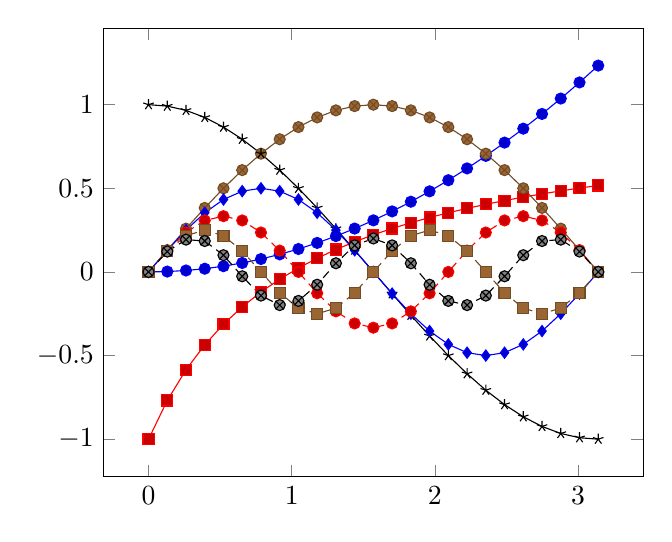
\begin{tikzpicture}
        \begin{axis}[domain=0:pi]
            \addplot+{x^2/8};
            \addplot+{(x-1)/(x+1)};
            \addplot+{sin(deg(x))};
            \addplot+{cos(deg(x))};
            \pgfplotsinvokeforeach{2,...,5}{
                \addplot+{1/#1*sin(#1*deg(x))};}
        \end{axis}
    \end{tikzpicture}
\end{minted}
\begin{center}
    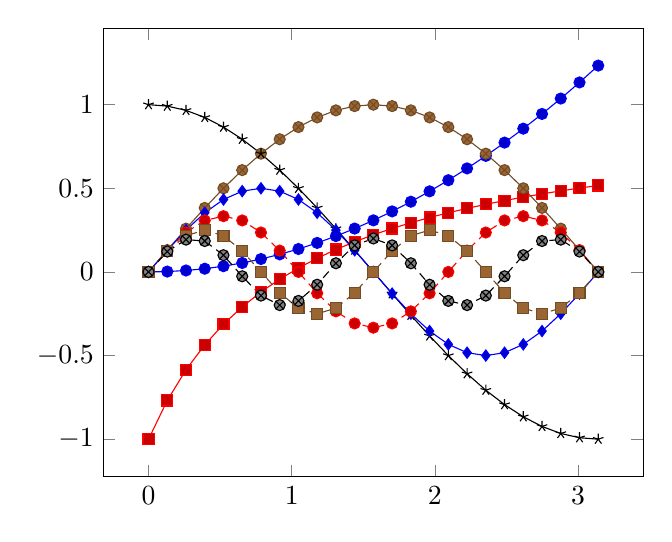
\begin{tikzpicture}
        \begin{axis}[domain=0:pi]
            \addplot+{x^2/8};
            \addplot+{(x-1)/(x+1)};
            \addplot+{sin(deg(x))};
            \addplot+{cos(deg(x))};
            \pgfplotsinvokeforeach{2,...,5}{
                \addplot+{1/#1*sin(#1*deg(x))};}
        \end{axis}
    \end{tikzpicture}
\end{center}

\paragraph{Asymptopes}
A notable addition made is some nice asymptote-related pgf keys that have been added.
There are three relevant keys
\begin{itemize}
    \item[] \mintinline{tex}{v asym} locations(s) of vertical asymptotes
    \item[] \mintinline{tex}{h asym} locations(s) of horizontal asymptotes
    \item[] \mintinline{tex}{asym gap} distance around vertical asymptote which is cleared
\end{itemize}

\begin{minipage}{\linewidth}
    \begin{minted}{tex}
        \begin{tikzpicture}
            \begin{axis}[domain=0:3,small]
                \addplot+[asym gap=0.05,v asym={0.5,1.5,2.5}]{tan(deg(pi*x))};
            \end{axis}
        \end{tikzpicture}
        \begin{tikzpicture}
            \begin{axis}[domain=-1:3,small]
                \addplot+[asym gap=0.1,v asym=1,h asym=5]{1/(x-1)+5};
            \end{axis}
        \end{tikzpicture}
    \end{minted}
    \begin{center}
        \begin{tikzpicture}
            \begin{axis}[domain=0:3,small]
                \addplot+[asym gap=0.05,v asym={0.5,1.5,2.5}]{tan(deg(pi*x))};
            \end{axis}
        \end{tikzpicture}
        \begin{tikzpicture}
            \begin{axis}[domain=-1:3,small]
                \addplot+[asym gap=0.1,v asym=1,h asym=5]{1/(x-1)+5};
            \end{axis}
        \end{tikzpicture}
    \end{center}
\end{minipage}

\section{Code}

This package spends a few lines tweaking
the minted and tcolorbox config to get code
blocks to look rather nice.

For example:
\begin{minted}[escapeinside=||,highlightlines={8,17}]{tex}
    \section{Code}

    This package spends a few lines tweaking
    the minted and tcolorbox config to get code
    blocks to look rather nice.

    For example:
    \begin{minted}[escapeinside=||,highlightlines={8,17}]{tex}
        \section{Code}

        This package spends a few lines tweaking
        the minted and tcolorbox config to get code
        blocks to look rather nice.

        For example:
        |\dots|
    \end||{minted}
\end{minted}

\section{Chemistry}
When the \mintinline{tex}{chem} option is used, \mintinline{tex}{mhchem}
is loaded with the configuration, however \mintinline{tex}{chemfig}
undergos a few modifications to make the results look cleaner.

\begin{center}
    \chemfig{*6(-=-(-COOH)=-=)}
    \chemfig{X-[1]=^[-1]-[1]-[-1]-[1]-[-1]=^[1]-[-1]}
    \qquad
    \chemfig{-[1](=[3]O)-[-1]}
\end{center}

\begin{minted}[firstnumber=310]{tex}
	\setchemfig{
		chemfig style={line width=0.06642 em},  % 'Line Width'
		angle increment=30,
		double bond sep=0.35700 em,  % 'Bond Spacing'
		atom sep=1.78500 em,  % 'Fixed Length'
		bond offset=0.18265 em  % 'Margin Width'
	}
	\renewcommand*\printatom[1]{\small\ensuremath{\mathsf{#1}}}
\end{minted}

\section{Links and Metadata}
\renewcommand{\ULthickness}{1pt}
\def\soutt{\bgroup \ULdepth=-.45ex \ULset}
Both the \mintinline{tex}{hyperref} and \mintinline{tex}{hyperxmp} packages are used.
The widely used hyperref package of course provides hyperlinks.
This is \soutt{ab}used to add a few extra links; specificly
every page number is a link to the TOC, and the text of every header
links to the relevant chapter page.
This allows you to jump all over the document in just a few clicks.

The hyperxmp package is rather handy for setting a few fields of pdf metadata.
Using the \mintinline{tex}{\title}, \mintinline{tex}{\author}, and \mintinline{tex}{\subtitle}
attributes it sets the relevant metadata fields.

\chapter{Boring Info}

\section{Implementation}

While originally one giant class file, each major component has now been split off
into a \mintinline{tex}{.sty} file that can also operate as a standalone package.
Currently, the following packages exist:
\begin{multicols}{2}
    \begin{itemize}
        \item bmc-boxes
        \item bmc-color
        \item bmc-fonts
        \item bmc-maths
        \item bmx-ref
        \item bmc-sectioning
    \end{itemize}
\end{multicols}

\section{Class Options}

This class builds off \mintinline{tex}{scrartcl},
any other options than those listed here will just be passed through.

\subsection{Main Styling}

\paragraph{\ttfamily dark}
Switches to a dark version of the style
\paragraph{\ttfamily solid}
Uses style with solid title page, and wide stripes on chapter pages, with solid colour bar at top of pages
\paragraph{\ttfamily stripe}
Uses plain background on title page, and thin stripes on chapter pages
\paragraph{\ttfamily article}
Use \mintinline{tex}{scrartcl} class instead of \mintinline{tex}{scrrept}
\paragraph{\ttfamily notes}
Move the margins to make room for notes

\subsection{Fonts}
\paragraph{Body Text}
Use \mintinline{tex}{[body=<variant>]}, where variant is one of  \mintinline{tex}{serif}, \mintinline{tex}{sans}, or \mintinline{tex}{mono}.
\\The default is \mintinline{tex}{serif}.

\paragraph{Math}
Use \mintinline{tex}{[math=<variant>]}, where variant is one of  \mintinline{tex}{serif}, \mintinline{tex}{sans}, or \mintinline{tex}{mono}.
\\The default is \mintinline{tex}{serif}.

\subsection{Headings}

These options set the style of the following components
\begin{itemize}
    \item \mintinline{tex}{\chapter} through to \mintinline{tex}{\subparagraph}
    \item The page head, and page number
    \item Caption labels
\end{itemize}

Use \mintinline{tex}{[headings=<variant>]}, where variant is one of  \mintinline{tex}{serif}, \mintinline{tex}{sans}, or \mintinline{tex}{mono}.
\\The default is \mintinline{tex}{sans}.

\subsection{Package Related}

\paragraph{\ttfamily chem}
Load and configure \mintinline{tex}{mhchem} and \mintinline{tex}{chemfig} packages

\paragraph{\ttfamily code}
Load and configure minted package

\paragraph{\ttfamily plot}
Load and configure \mintinline{tex}{pgfplots} package

\paragraph{\ttfamily math}
Load and configure some mathematical packages, and set font to match main text font (also see \mintinline{tex}{math-serif} etc.)

\newpage
\section{Packages Used}

\subsection{Overview}

\begin{table}[!htb]
    \centering
    \small
    \setlength{\tabcolsep}{0pt}
    \renewcommand{\arraystretch}{1.3}
    \begin{tabular}{>{\hspace{3pt}\normalsize}l>{\hspace{5pt}}*{5}{p{7.9em}}l}
        \toprule
        Category & \multicolumn{5}{l}{\normalsize Packages} \\
        \midrule
        General & \hyperref[par:etoolbox]{etoolbox} & \hyperref[par:xpatch]{xpatch} & \hyperref[par:Silence]{Silence} & \hyperref[par:ifdraft]{ifdraft} & \hyperref[par:geometry]{geometry}  \\
        & \hyperref[par:titlesec]{titlesec} & \hyperref[par:titletoc]{titletoc} & \hyperref[par:framed]{framed} & \hyperref[par:textpos]{textpos} & \hyperref[par:calc]{calc} \\
         & \hyperref[par:xcolor]{xcolor} & \hyperref[par:tikz]{tikz} & \hyperref[par:hyperref]{hyperref} & \hyperref[par:hyperxmp]{hyperxmp} & \hyperref[par:scrlayer-scrpage]{scrlayer-scrpage} \\
        Text & \hyperref[par:microtype]{microtype} & \hyperref[par:setspace]{setspace} & \hyperref[par:plex-serif]{plex-serif} & \hyperref[par:plex-sans]{plex-sans} & \hyperref[par:plex-mono]{plex-mono} \\[4pt]
        & \hyperref[par:multicol]{multicol} & \\
         Table & \hyperref[par:booktabs]{booktabs} & \hyperref[par:tabularx]{tabularx} & \hyperref[par:longtable]{longtable}  \\[4pt]
         Graphics & \hyperref[par:graphicx]{graphicx} & \hyperref[par:grffile]{grffile} & \hyperref[par:subcaption]{subcaption} & \hyperref[par:caption]{caption} \\[4pt]
         infoBulle & \hyperref[par:infoBulle]{infoBulle} & \hyperref[par:marginInfoBulle]{marginInfoBulle} & \hyperref[par:fontawesome5]{fontawesome5}\\[4pt]
         Chemistry & \hyperref[par:mhchem]{mhchem} & \hyperref[par:chemfig]{chemfig} \\[4pt]
         Code & \hyperref[par:minted]{minted} & \hyperref[par:tcolorbox]{tcolorbox} \\[4pt]
         Math & \hyperref[par:amssymb]{amsmath} & \hyperref[par:amssymb]{amssymb} & \hyperref[par:mathdesign]{mathdesign} & \hyperref[par:xfrac]{xfrac} & \hyperref[par:cancel]{cancel} \\[4pt]
         & \hyperref[par:mathtools]{mathtools} & \hyperref[par:mathastext]{mathastext} & \hyperref[par:pgfplots]{pgfplots} \\
         \bottomrule
    \end{tabular}
    \caption{All Packages Used by This Class}
    \label{table:all-packages}
\end{table}

\subsection{General Packages}

\paragraph{\ttfamily etoolbox}\label{par:etoolbox}
Provides LaTeX frontends to some of the new primitives provided by e-TeX
as well as some rather useful some generic tools --- namely,
\begin{itemize}
    \item Robust definitions
    \item Command Patching
    \item Command Protection
    \item Arithmetic counters and lengths
    \item Document Hooks
    \item Environment Hooks
\end{itemize}
\paragraph{\ttfamily xpatch}\label{par:xpatch}
Extends the command patching provided by \hyperref[par:etoolbox]{etoolbox}
\paragraph{\ttfamily Silence}\label{par:Silence}
Allows me to ignore expected warnings.
\paragraph{\ttfamily ifdraft}\label{par:ifdraft}
To make it easy to change things up a bit more than usual for draft mode.
\paragraph{\ttfamily scrlayer-scrpage}\label{par:scrlayer-scrpage}
To allow for those lovely headers and footers.
\paragraph{\ttfamily geometry}\label{par:geometry}
Loaded with options,
\begin{minted}[firstnumber=452]{tex}
    a4paper, ignoreheadfoot, left=\leftmargin, right=\rightmargin, top=2cm, bottom=3.5cm, headsep=1cm
\end{minted}
\paragraph{\ttfamily titlesec}\label{par:titlesec}
Allows for customisation of \mintinline{tex}{\chapter} etc.
Was originally used for all section commands, but now all except for
\mintinline{tex}{\chapter} have been transitioned to KOMA-script.
\paragraph{\ttfamily titletoc}\label{par:titletoc}
Allows significant tweaking to how the table of contents looks.
\paragraph{\ttfamily framed}\label{par:framed}
Facilitate the definition of new environments that take multi-line material, wrap it with some
non-breakable formatting (some kind of box or decoration) and allow page breaks in the material
\paragraph{\ttfamily textpos}\label{par:textpos}
Facilitates placement of boxes at absolute positions on the LaTeX page.
Loaded with options \mintinline{tex}{absolute,overlay}
\paragraph{\ttfamily hyperref}\label{par:hyperref}
Used to produce all sorts of hyperlinks in a document.
Loaded with option \mintinline{tex}{pdfa}
\paragraph{\ttfamily hyperxmp}\label{par:hyperxmp}
Improves metadata setting with hyperref.
\paragraph{\ttfamily calc}\label{par:calc}
Adds infix expressions to perform arithmetic on the arguments of the LaTeX commands
\mintinline{tex}{\setcounter}, \mintinline{tex}{\addtocounter}, \mintinline{tex}{\setlength}, and \mintinline{tex}{\addtolength}
\paragraph{\ttfamily xcolor}\label{par:xcolor}
Provides all sorts of colour use and mixing capabilities.
\paragraph{\ttfamily tikz}\label{par:tikz}
It's tikz. You can't draw anything without it.

\subsection{Text}

\paragraph{\ttfamily microtype}\label{par:microtype}
Always good to have. It simply makes text look better, specificity it applies the following,
\begin{itemize}
    \item Character protrusion
    \item Font expansion
    \item Adjustment of interword spacing and kerning
    \item Letterspacing
\end{itemize}
Configured with,
\begin{minted}[firstnumber=67]{tex}
activate={true,nocompatibility}, final, tracking=true, kerning=true, spacing=true, factor=2000
\end{minted}
\paragraph{\ttfamily plex-serif}\label{par:plex-serif}
\paragraph{\ttfamily plex-sans}\label{par:plex-sans}
\paragraph{\ttfamily plex-mono}\label{par:plex-mono}
\paragraph{\ttfamily setspace}\label{par:setspace}
Provides an easy way to set line spacing with commands such as
\mintinline{tex}{\doublespacing} and \mintinline{tex}{\setstretch{1.25}}.
\paragraph{\ttfamily multicol}\label{par:multicol}
Split text into multiple columns (up to 10).

\subsection{Table-related}

\paragraph{\ttfamily booktabs}\label{par:booktabs}
Contribues different width \mintinline{tex}{\hline} variants.
\paragraph{\ttfamily tabularx}\label{par:tabularx}
Adds the \mintinline{tex}{tabularx} environment which has its width explicitly set,
\mintinline{tex}{X} column type which automatically determines its width based on its contents.
\paragraph{\ttfamily longtable}\label{par:longtable}
Provides a good way of allowing tables to spread over multiple pages.

\subsection{Graphics and Figures}

\paragraph{\ttfamily graphicx}\label{par:graphicx}
Makes loading images (\mintinline{tex}{includegraphics}) work well.
\paragraph{\ttfamily grffile}\label{par:grffile}
This fixes the fix allowed filenames of graphicx.
\paragraph{\ttfamily caption}\label{par:caption}
Provides many ways to customise the captions in floating environments like figure and table,
and cooperates with many other packages.
Facilities include rotating captions, sideways captions, continued captions (for tables or figures that come in several parts).
Loaded with option \mintinline{tex}{hypcap=true}
\paragraph{\ttfamily subcaption}\label{par:subcaption}
Allows for typesetting of sub-figures and sub-tables.

\subsection{infoBulle}

\paragraph{\ttfamily fontawesome5}\label{par:fontawesome5}
Fontawesome 5, need I say any more?
\paragraph{\ttfamily infoBulle}\label{par:infoBulle}
\paragraph{\ttfamily marginInfoBulle}\label{par:marginInfoBulle}

\subsection{Chemistry}

\paragraph{\ttfamily mhchem}\label{par:mhchem}
Useful for simple inline chemistry.
\paragraph{\ttfamily chemfig}\label{par:chemfig}
Useful for chemical diagrams.

\subsection{Code}

\paragraph{\ttfamily minted}\label{par:minted}
Configured as follows,
\begin{minted}[firstnumber=476]{tex}
\setminted{
    frame=none,
    % framesep=2mm,
    baselinestretch=1.2,
    fontsize=\footnotesize,
    highlightcolor=page!95!text!80!primary,
    linenos,
    breakanywhere=true,
    breakautoindent=true,
    breaklines=true,
    tabsize=4,
    xleftmargin=3.5em,
    autogobble=true,
    obeytabs=true,
    python3=true,
    % texcomments=true,
    framesep=2mm,
    breakbefore=\\\.+,
    breakafter=\,
}
\end{minted}

\paragraph{\ttfamily tcolorbox}\label{par:tcolorbox}
Used for prettifying the \mintinline{tex}{minted} environment.
Loaded with option \mintinline{tex}{many}

\subsection{Maths Related}
These packages are loaded by the \mintinline{tex}{math}
option (or one of its derivatives).

\paragraph{\ttfamily amsmath,amssymb}\label{par:amssymb}
Extends the maths commands and symbols in latex.
\paragraph{\ttfamily mathdesign}\label{par:mathdesign}
To use the Utopia font for maths symbols.
\paragraph{\ttfamily xfrac}\label{par:xfrac}
Allows split level fractions \(*\sfrac{a}{b}\) better than \mintinline{tex}{{}^{a}/{}_{b}} can produce.
\paragraph{\ttfamily cancel}\label{par:cancel}
Allows for easy cancelling within math like so ---
\(*\cancel{\eta}\) and \(*\cancelto{0}{\eta}\).
Loaded with option \mintinline{tex}{makeroom}
\paragraph{\ttfamily mathtools}\label{par:mathtools}
Provides a variety of enhancements to make maths \emph{even} better.
\begin{itemize}
    \item Extensible symbols, such as brackets, arrows, harpoons, etc.;
    \item Various symbols such as \mintinline{tex}{\coloneqq} (\(*\coloneqq\));
    \item Easy creation of new tag forms;
    \item Showing equation numbers only for referenced equations;
    \item Extensible arrows, harpoons and hookarrows;
    \item Starred versions of the amsmath matrix environments for specifying the column alignment;
    \item More building blocks: multlined, cases-like environments, new gathered environments;
    \item Maths versions of \mintinline{tex}{\makebox}, \mintinline{tex}{\llap}, \mintinline{tex}{\rlap} etc.;
    \item Cramped maths styles; and more\dots
\end{itemize}
\paragraph{\ttfamily mathastext}\label{par:mathastext}
Uses relevant plex font for maths letters.
Uses options \mintinline{tex}{basic,italic,symbolgreek}.

\paragraph{\ttfamily pgfplots}\label{par:pgfplots}
Loaded by the \mintinline{tex}{plot} option.

\section{Configuration}

\subsection{Colours}
\label{subsec:config-colours}
\clearrow
\begin{longtable}{l>{\rowmac}p{10em}>{\rowmac}p{10em}}
    \toprule
    Name & Default (Light) & Default (Dark) \\
    \midrule
    \endfirsthead
    \toprule
    \setrow{\scriptsize} Name & Default (Light) & Default (Dark) \clearrow \\
    \midrule
    \multicolumn{1}{c}{\scriptsize\vdots} & \multicolumn{1}{c}{\scriptsize\vdots} & \multicolumn{1}{c}{\scriptsize\vdots} \\
    \endhead
    \multicolumn{1}{c}{\scriptsize\vdots} & \multicolumn{1}{c}{\scriptsize\vdots} & \multicolumn{1}{c}{\scriptsize\vdots} \\
    % \midrule
    \bottomrule
    \endfoot
    \bottomrule
    \endlastfoot
    \mintinline{tex}{text} & \#000000 & \#FCFCFC \\
    \mintinline{tex}{page} & \#FFFFFF & \#222222 \\
    \mintinline{tex}{href} & tertiary & secondary \\
    \mintinline{tex}{primaryVariant} & primary\linebreak[0]!75!Cream\linebreak[0]>twheel,-3,360 & \ditto \\
    \mintinline{tex}{inlinemath} & secondary\linebreak[0]!50!text & tertiary\linebreak[0]!50!text \\
    \rowcolor{tableheadcolor}
    \multicolumn{2}{l}{\fontseries{l}\selectfont infoBulle} & \\
    \hiderowcolors
    \mintinline{tex}{infoBulleBackground} & page!90!text & \ditto \\
    \mintinline{tex}{infoBulleText} & text & \ditto \\
    \mintinline{tex}{marginInfoBulleBackground} & page & \ditto \\
    \mintinline{tex}{marginInfoBulleText} & text & \ditto \\
    \mintinline{tex}{criticalColor} & Red & \ditto \\
    \mintinline{tex}{questionColor} & Purple & \ditto \\
    \mintinline{tex}{informationColor} & Green & \ditto \\
    \mintinline{tex}{checkColor} & Blue & \ditto \\
    \mintinline{tex}{warningColor} & Orange & \ditto \\
    \mintinline{tex}{tipColor} & Purple & \ditto \\
    \mintinline{tex}{exampleColor} & Blue & \ditto \\
    \mintinline{tex}{mathematicalColor} & Orange & \ditto \\
    \mintinline{tex}{codeColor} & Grey & \ditto \\
\end{longtable}

\subsection{Palettes}
\label{subsec:palettes}
The module \mintinline{tex}{bmc-color} has a few inbuilt pallets
sourced from \url{https://flatuicolors.com}.
Using the relevant country code (see website) you can select a palette two ways:
\begin{enumerate}
    \item Passing the palette as an option when loading, \mintinline{tex}{[palette=<palette code>]}
    \item Setting the palette via \mintinline{tex}{\usepalette{<palette code>}}
\end{enumerate}
The second method can be employed anywhere in the document.

\subsubsection{Creating Your Own Palette}

Palettes can be created with the command \mintinline{tex}{\newpalette{<palette code>}{<colour definitions>}}.
The `colour definitions' simply consist of any \mintinline{tex}{xcolor} commands that define the colour.
You may wonder why not just define your own macro for your colours ---
this method provides two minor features that may prove useful depending on the situation.
\begin{itemize}
    \item `Main' colours (e.g.\ Red, Green\dots) not provided are populated from a default (\texttt{de})
    \item `Derived' colours (e.g.\ LightRed, DarkGreen) are mixed from main colours if not given
\end{itemize}
It is a good idea to provide colours from the following list, however you can provide as many or as few
colours as you like.

\begin{center}
    % \em
    \fontseries{tx}\selectfont
    \textcolor{Black!50!text}{Black},
    \textcolor{White!50!text}{White},
    \textcolor{Cream!50!text}{Cream},
    \textcolor{Grey!50!text}{Grey},
    \textcolor{Red!50!text}{Red},
    \textcolor{Yellow!50!text}{Yellow},
    \textcolor{Blue!50!text}{Blue},
    \textcolor{Green!50!text}{Green},
    \textcolor{Orange!50!text}{Orange},
    \textcolor{Purple!50!text}{Purple},
    \textcolor{Cyan!50!text}{Cyan}.
    \\[0.5ex]
    \fontseries{l}\selectfont
    \upshape\scriptsize\slshape
    Note: All except for Black, White, and Cream have the
    accompanying Light and Dark variants.
\end{center}

\newpage
\subsubsection{Default Pallets}
\newcommand{\colorBoxSmallBW}{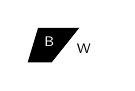
\begin{tikzpicture}[baseline=0.6ex,x=2.5em,y=2.5em]
    \fill[Black] (0,0) -- (0.15,0.5) -- (0.75,0.5) -- (0.35,0) -- cycle;
    \fill[White] (0.35,0) -- (0.75,0.5) -- (1.15,0.5) -- (1,0) -- cycle;
    \node[text width=2] at (0.28,0.3) {\tiny\color{White}\textsf{B}};
	\node[text width=2] at (0.75,0.2) {\tiny\color{Black}\textsf{W}};
\end{tikzpicture}%
\hspace{-0.375em}}
% \newcommand{\triag}{%
%     \begin{tikzpicture}[baseline=0.6ex,x=2.5em,y=2.5em]
%     \end{tikzpicture}%
%     \hspace{-1.5em}}
\newcommand{\colorBoxSmallLD}[2][]{%
    \hspace{-0.75em}%
    \begin{tikzpicture}[baseline=0.6ex,x=2.5em,y=2.5em]
    \fill[White] (-0.75,-0.4) -- (-0.45,0.5) -- (1.15, 0.5) -- (0.8875, -0.4) -- cycle;
    \if1#1\fill[page] (-0.75,-0.4) -- (-0.62,0) -- (-0.12, -0.4) -- cycle;\fi
    \fill [#2] (0, 0) rectangle (1, 0.5);
    \fill[Light#2] (0,0) -- (0.15,0.5)-- (0,0.5) -- (-0.15,0) -- cycle;
    \fill[Dark#2] (1,0.5) -- (0.85,0) -- (1,0) -- (1.15,0.5) -- cycle;
	\node[text width=2,align=center] at (0.2,-0.2) {\tiny\color{#2}\textsf{\fontseries{tx}\selectfont#2}};
\end{tikzpicture}}

\newcommand{\colorBoxSmallLDs}[2][]{%
    \begin{tikzpicture}[baseline=0.6ex,x=2.5em,y=2.5em]
        \fill [#2] (0, 0) rectangle (1, 0.5);
        \fill[Light#2] (0,0) -- (0.4,0) -- (0,0.25) -- cycle;
        \fill[Dark#2] (1,0.5) -- (0.6,0.5) -- (1,0.25) -- cycle;
	\node[text width=2,align=center] at (0.2,-0.2) {\tiny\color{#2}\textsf{\fontseries{tx}\selectfont#2}};
\end{tikzpicture}}

\newcommand{\demoPalette}[2][]{
    \vspace{-1.8ex}
    \usepalette{#2}
    \paragraph{\rlap{\texttt{#2}}\hspace*{3em}}
    \colorBoxSmallBW{}
    \colorBoxSmallLD[1]{Grey}%
    % \triag%
    \colorBoxSmallLD{Red}%
    \colorBoxSmallLD{Blue}%
    \colorBoxSmallLD{Green}%
    \colorBoxSmallLD{Yellow}%
    \colorBoxSmallLD{Orange}%
    \colorBoxSmallLD{Purple}%
    \colorBoxSmallLD{Cyan} \\[-1.8ex]
    {\scriptsize\sffamily #1}
    \vspace{-1ex}
}
\vspace{2ex}
\demoPalette[German \fontseries{l}\selectfont (default)]{de}
\demoPalette[FlatUI]{fui}
\demoPalette[Australian]{au}
\demoPalette[American]{us}
\demoPalette[British]{uk}
\demoPalette[Canadian]{ca}
\demoPalette[Chinese]{cn}
\demoPalette[Dutch]{nl}
\demoPalette[French]{fr}
\demoPalette[Indian]{in}
\demoPalette[Russian]{ru}
\demoPalette[Spanish]{es}
\demoPalette[Swedish]{se}
\demoPalette[Turkish]{tr}

{\color{primary}\rule{\textwidth}{.2mm}}

\demoPalette[Solarized]{sol}
\demoPalette[Monokai]{mon}

\usepalette{de}

\chapter{Reasoning}

\section{Layout}



\section{Typefaces}
\label{sec:why-typefaces}

\subsection{Studies}
Unfortunately large type studies on UI/UX and typography
seem to be exclusive to large companies that care about this
(e.g.\ microsoft, google, etc.) and don't seem to publish their results.

It has long been known that there is a relationship between the reader's judged
aesthetic pleasingness of text, and the legibility (\cite{Tinker_Paterson_1942}).
Regardless of the underlying mechanisms, this provides strong justification for
putting in the effort to make a document have good content, \emph{and} good aesthetics.

A study by \cite{kaspar2015matter} presented subjects with research papers in
serif and sans-serif fonts. They found that sans-serif fonts increase reading speed.
While this was not a focus of the study, it is apparently in line with previous research.
A 2005 study by~\cite{Gasser_Boeke_Haffernan_Tan_2005} found that
sans-serif founts produced 9\% improvement in recall (\(N=149\), \(p=0.05\)).

While~\cite{kaspar2015matter} found that while sans-serif fonts are read faster,
in every category tested, sans-serif fonts performed better. Specially serifs were
found to improve:
\begin{itemize}
    \item Comprehension
    \item Interest in paper and appeal of abstract
    \item Perceived quality and importance
\end{itemize}

More generally,~\cite{larson2007measuring} identified two measures that
successfully indicate aesthetic difference. Performance of creative cognitive tasks
after reading a document, and subconscious activation of the facial muscle
responsible for frowning. For both measures a method that had \(p=0.04\) was yielded.
It is rather interesting that they found that improved typography reduced frowning
and and improved creative cognitive task performance.

Semantic associations between the typeface chosen and the content also seem to be
important. \cite{web_chooserightfont} appears to give a good overview of this.

\subsection{The Elements of Typographic Style}
While, as demonstrated previously, there are \textit{some} studies about typefaces,
they are few and far between, done on a small scale, and rarely reproduced.
Hence one of the best resources for typographic guidances is eminent publications
on the matter. \citetitle{Bringhurst_2004} is one of the foremost books, widely held
in high esteem. Reading through it there a several useful suggestions which I have
tried to implement here.

\paragraph{Conclusions from \P~3.2.2}
With some acronyms each letter is pronounced individually (such as the \acr{ISO}
or \acr{GNU}). To achieve this effect typographically spaced small caps are very
useful. They are also useful in a variety of other situations, for example:
\begin{center}
    \acr{WWII} formally ended at 12:00 \acr{AM} on 8 May nineteen forty-five \acr{AD}. \\
    WWII formally ended at 12:00 AM on 8 May nineteen forty-five AD\@.
\end{center}
The general rule given is --- \emph{`For abbreviations and acronyms in the midst of normal
text, use spaced small caps'}.

\paragraph{Conclusions from \P~4.4.1}
With regard to tables
\begin{enumerate}
    \item Avoid shrinking font size
    \item Minimise `furniture' (rules,boxes,dots, etc.)
    \item Rules / tint blocks, when absolutely necessary, should run in the
    reading direction
    \item Rules along the (vertical) outside of the table are useless
    \item Ensure sufficient white space is maintained
\end{enumerate}

\paragraph{Conclusions from \P~4.5.1}
Short texts, such as research papers generally don't benefit from much padding
at the start and end. The same does \emph{not} apply to books.
As such \gls{bmc} implements two \mintinline{tex}{\maketitle}s.
The default full page one seen on this document, and a shorter one used when the
\mintinline{tex}{article} option is passed to the class.

\paragraph{Conclusions from \P~5.1.3}
Use the ampersand (\&) in heads and titles.

\paragraph{Conclusions from \P~5.1.4}
Line-end hyphens best lie in the right margin. This is achieved by use of the
\mintinline{tex}{factor=2000} option with the microtype package.

\section{Colour}

\printbibliography
\printglossary

\end{document}

